% Part: counterfactuals
% Chapter: minimal-change-semantics
% Section: introduction

\documentclass[../../../include/open-logic-section]{subfiles}

\begin{document}

\olfileid{cnt}{min}{int}

\olsection{Introduction}

Stalnaker and Lewis proposed accounts of counterfactual conditionals
such as ``If the match were struck, it would light.''  Their accounts
were proposals for how to properly nderstand the truth conditions for
such sentences. The idea behind both proposals is this: to evaluate
whether a counterfactual conditional is true, we have to consider
those possible worlds which are minimally different from he way the
world actually is to make the antecednet true. If the consequent is
true in these possible worlds, then the counterfactual is true. For
instance, suppose I hold a match and a matchbook in my hand. In the
actual world I only look at them and ponder what would happen if I
were to strike the match. The minimal change from the actual world
where I strike the match is that where I decide to act and strike the
match. It is minimal in that nothing else changes: I don't also jump
in the air, striking the match doesn't also light my hair on fire, I
don't suddenly lose all strenght in my fingers, I am not simultaneously
doused with water in a SuperSoaker ambush, etc. In that alternative
possibility, the match lights. Hence, it's true that if I were to
strike the match, it lights.

This intuitive account can be paired with formal semantics for logics
of counterfactuals.  Lewis introduced the symbol ``$\boxright$'' for
the counterfactual, and Stalnaker used~``$>$''. We'll use~$\cif$, and
add it as a binary connective to propositional logic. So, we have, in
addition to !!{formula}s of the form $!A \lif !B$ also !!{formula}s of
the form~$!A \cif !B$. The formal semantics, like the relational
semantics for modal logic, is based on models in which !!{formula}s
are evaluated at worlds, and the satisfaction condition defining
$\mSat{M}{!A \cif !B}[w]$ is given in terms of $\mSat{M}{!A}[w']$ and
$\mSat{M}{!B}[w']$ for some (other) worlds~$w'$. Which $w'$?
Intuitively, the one(s) closest to~$w$ for which it holds
that~$\mSat{M}{!A}[w']$. This requires that a relation of
``closeness'' has to be included in the model as well.

Lewis introduced an instructive way of representing counterfactual
situations graphically. Each possible world is at the center of a set
of nested spheres containing other worlds---we draw these spheres as
concentric circles. The worlds between two spheres are equally close
to the world at the center as each other, those contained in a nested
sphere are closer, and those in a surrounding sphere further away.
\begin{center}
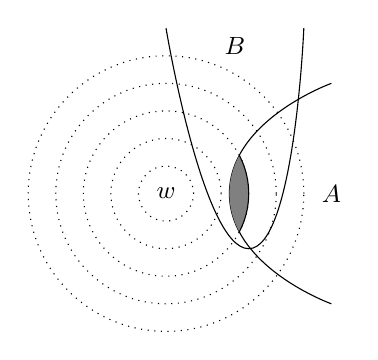
\begin{tikzpicture}[scale=.7]\small
  \draw[dotted] (0,0) node {$w$} circle (.5) circle (1)
  circle (1.5) circle (2) circle (2.5);
  \begin{scope}
    \draw[clip] plot [smooth,tension=1.2] coordinates { (3,2) (1.15,0) (3,-2)};
    \filldraw[fill=gray] (0,0) circle (1.5);
  \end{scope}
  \draw plot [smooth,tension=1.2] coordinates {(0, 3) (1.5,-1) (2.5,3)};
  \path (1.25,3) node[below] {$\formula{B}$};
  \path (3,0) node {$\formula{A}$};
\end{tikzpicture}
\end{center}
The closest $!A$-worlds are those worlds $w'$ where~$!A$ is satisfied
which lie in the smallest sphere around the center world~$w$ (the gray
area). Intuitively, $!A \cif !B$ is satisfied at $w$ if $!B$ is true
at all closest $!A$-worlds.

\end{document}
